\documentclass[tikz,border=10pt]{standalone}
\usetikzlibrary{calc, angles, quotes, decorations.pathmorphing, decorations.markings}

\begin{document}
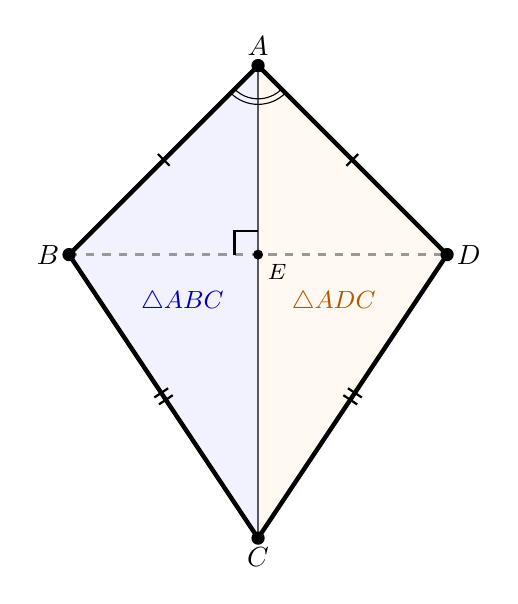
\begin{tikzpicture}[>=stealth, scale=1.2]

  % Styles for tick marks
  \tikzset{
    ticks/.style={
      postaction={decorate},
      decoration={
        markings,
        mark=at position 0.5 with {\draw[thick] (0,-3pt) -- (0,3pt);}
      }
    },
    double ticks/.style={
      postaction={decorate},
      decoration={
        markings,
        mark=at position 0.5 with {
          \draw[thick] (-1.5pt,-3pt) -- (-1.5pt,3pt);
          \draw[thick] (1.5pt,-3pt) -- (1.5pt,3pt);
        }
      }
    }
  }

  % Coordinates for Kite ABCD
  \coordinate (A) at (0,3);
  \coordinate (B) at (-2,1);
  \coordinate (D) at (2,1);
  \coordinate (C) at (0,-2);
  \coordinate (E) at (0,1); % Intersection of diagonals

  % Fill the two congruent structural triangles to show the SSS symmetry
  \fill[blue!5] (A) -- (B) -- (C) -- cycle;
  \fill[orange!5] (A) -- (D) -- (C) -- cycle;

  % Draw Diagonals first so they sit cleanly underneath points
  \draw[thick, dashed, gray!80] (B) -- (D);
  \draw[thick, gray!70!black] (A) -- (C);

  % Draw Outer Sides with Congruence Ticks
  \draw[ultra thick, ticks] (A) -- (B);
  \draw[ultra thick, ticks] (A) -- (D);
  \draw[ultra thick, double ticks] (C) -- (B);
  \draw[ultra thick, double ticks] (C) -- (D);

  % Perpendicular Right Angle Mark at E
  \draw[thick] ($(E)+(0,0.25)$) -- ($(E)+(-0.25,0.25)$) -- ($(E)+(-0.25,0)$);

  % Vertices
  \fill (A) circle (2pt) node[above] {$A$};
  \fill (B) circle (2pt) node[left] {$B$};
  \fill (C) circle (2pt) node[below] {$C$};
  \fill (D) circle (2pt) node[right] {$D$};
  \fill (E) circle (1.5pt) node[below right, font=\footnotesize] {$E$};

  % Symmetric Angle Markers
  \draw pic[draw, angle radius=12pt] {angle = B--A--C};
  \draw pic[draw, angle radius=14pt] {angle = B--A--C};

  \draw pic[draw, angle radius=12pt] {angle = C--A--D};
  \draw pic[draw, angle radius=14pt] {angle = C--A--D};

  % Labels/Annotations
  \node[text=blue!70!black, font=\small] at (-0.8, 0.5) {$\triangle ABC$};
  \node[text=orange!70!black, font=\small] at (0.8, 0.5) {$\triangle ADC$};

\end{tikzpicture}
\end{document}
